\chapter{二维基于紧致埃尔米特重构的双曲守恒律两步四阶数值格式}
\label{sec:2D-method}

在\cref{sec:framework}中,
我们为了使用紧致的埃尔米特重构,
提出了改进的两步四阶时间推进框架。
在本章,
我们将基于此框架设计二维基于紧致埃尔米特重构的基本无振荡的两步四阶数值格式,
所以我们需要选择适当的重构算法和解法器。

\section{广义黎曼问题解法器}
\label{sec:2D-solver-sec4}

在二维情形下,
本文采用二维的Godunov解法器和文\cite{GRP_qi}中的二维弱耦合的广义黎曼问题解法器作为标准一阶LW型解法器,
然后使用\cref{sec:2D-Solver}中的线性二阶LW型解法器。
这些二维解法器和一维解法器的区别在于面对的黎曼问题和广义黎曼问题是不同的。
这里以高斯点$(x_{i+\frac{1}{2}},y_{j+G})$为例,
并将$(x_{i+\frac{1}{2}},y_{j+G},t^n)$平移到原点,
二维的广义黎曼问题是
\begin{equation}
  \label{eq:2D-GRP}
  \left\{
  \begin{aligned}
     & {\partial_{t}}{\bm{u}} + {\partial_{x}}{\bm{f}}({\bm{u}}) + {\partial_{y}}{\bm{g}}({\bm{u}}) = 0, \\
     & {\bm{u}}(x,y,0) =
    \begin{cases}
      {\bm{u}}_{(i+\frac{1}{2},-),j+G}^n + \left({\partial_{x}}{\bm{u}}\right)_{(i+\frac{1}{2},-),j+G}^n x + \left({\partial_{y}}{\bm{u}}\right)_{(i+\frac{1}{2},-),j+G}^n y, & x<0,  \\
      {\bm{u}}_{(i+\frac{1}{2},+),j+G}^n + \left({\partial_{x}}{\bm{u}}\right)_{(i+\frac{1}{2},+),j+G}^n x + \left({\partial_{y}}{\bm{u}}\right)_{(i+\frac{1}{2},+),j+G}^n y, & x>0.
    \end{cases}
  \end{aligned}
  \right.
\end{equation}

由于二维情形下的解法器过于复杂,
这里就不做详细介绍,
读者如果有兴趣,
详见文献\cite{GRP_qi}。

\section{线性紧致埃尔米特重构及其相应的两步四阶格式}
\label{sec:2D-linear-rec}

在一维情形下,
因为文\cite{du2018hermite}中五阶HWENO重构相比四阶重构不够紧致,
同时计算开销更大,
所以我们新构造了四阶精度的紧致埃尔米特重构。
在二维情形下,
我们出于同样的原因,
不使用文\cite{du2018hermite}中逐维的HWENO5和WENO5重构,
而是尝试将一维的紧致埃尔米特重构推广到二维情形,
同时保持类似的性能。
另外,
逐维的重构不能保证对称性,
内存需求高,
还难以推广到非规则网格与非结构网格。

在本节,
我们将探讨二维情形下的线性埃尔米特重构。
我们希望这种重构比逐维的HWENO5和WENO5重构更加紧致,
希望它是四阶的,
更适合改进的两步四阶时间推进框架,
并且希望它是真正二维的。

给定一个函数$u(x,y)$,
定义函数$u(x,y)$及其导数$\nabla u = (v, w)$在计算单元$I_{ij}$上的平均值为
\begin{equation}
  {\overline{u}}_{ij} = \frac {1}{h_xh_y} \int_{I_{ij}} u(x,y)dx dy, \quad
  \left({\overline{v}}_{ij},{\overline{w}}_{ij}\right) = \frac {1}{h_xh_y} \int_{I_{ij}} \nabla u(x,y)dx dy,
\end{equation}
其中,
计算单元$I_{ij}=[x_{i-\frac 12},x_{i+\frac 12}]\times[y_{j-\frac 12},y_{j+\frac 12}]$,
其大小为$h_x=x_{i+\frac 12}-x_{i-\frac 12}$,
$i=1,\cdots, N_x$和$h_y=y_{j+\frac 12}-y_{j-\frac 12}$,
$j=1,\cdots, N_y$,
并且为了简单起见,
我们仍采用均匀网格。
同时也适用于非均匀网格。
对于$2k$阶重构,
我们希望在$k^2$个潜在的候选模板
\begin{equation}
  S^k_{rs}(i,j)=\bigcup_{m=0}^{k-1} \bigcup_{\ell=0}^{k-1} I_{i-r+m,j-s+\ell}, \quad
  r,s=0,1,\cdots,k-1,~k \ge 1,
\end{equation}
中选择适当的模板并在其上得到相应的埃尔米特重构$p^{rs}_{ij}(x,y)$,
其中的上标$r$和$s$表示这些值取决于模板$S^k_{rs}(i,j)$,
在没有引起歧义的情况下将被省略。

\subsection{线性紧致埃尔米特重构模板的选择策略}
\label{sec:2D-linear-rec-aim}

在这一小节,
我们会讨论对二维线性重构的要求。

\begin{enumerate}
  \item 我们所期望构造的线性紧致埃尔米特重构,
        应该在每个单元$I_{ij}$内以$2k$阶的精度近似$u(x,y)$,
        \begin{equation}
          p_{ij}(x,y) = u(x,y)+{\mathcal{O}}(h^{2k}),
        \end{equation}
        并且它的各阶导数满足
        \begin{equation}
          {\partial_{x}^{d_1}}{\partial_{y}^{d_2}}p_{ij}(x,y) = {\partial_{x}^{d_1}}{\partial_{y}^{d_2}}u(x,y)+{\mathcal{O}}(h^{2k-d_1-d_2}), \quad
          d_1+d_2 \le 2k-1.
        \end{equation}
        此时,
        我们可以得到,
        在单元边界的高斯点上,
        重构有$2k$阶近似精度。
  \item 我们希望构建的二维重构在一维问题中可以退化到我们在\cref{sec:1D-linear-rec}中给出的一维重构。
        这可以有效保障我们的二维重构可以取得类似一维重构的良好性能。
  \item 我们注意到,
        模板$S^k_{rs}$包含总共$k^2$个单元中的$3k^2$个自由度。
        而在$\mathcal{P}^{2k-1}$空间中,
        构造一个$2k$阶的重构只需要$2k^2+k$个自由度。
        当$k=1$时,
        两者是相等的,
        但当$k>1$时,
        存在冗余的自由度,
        这可能需要最小二乘法或其他技术。
        然而,
        我们认为最小二乘法的计算成本相当高,
        所以我们寻求另一种解决方案。
        我们将会忽略其中$k^2-k$个自由度,
        使得自由度可以刚好构造一个$2k$阶的重构。
  \item 我们需要使最终的模板尽可能对称。
  \item 此外,
        要确保目标单元$I_{ij}$本身在模板中。
\end{enumerate}

\subsection{线性紧致埃尔米特重构的具体形式}

我们综合\cref{sec:2D-linear-rec-aim}中的要求,
得到如下模板。

\begin{enumerate}
  \item 在$k=1$的情形下,
        唯一的模板选择如\cref{subfig:stencil1} 所示。
        在这个图中,
        单元平均值$\bar u_{ij}$由一个圆圈表示,
        而导数平均值$\bar v_{ij}$或$\bar w_{ij}$由一个相应方向的箭头表示。
        从此模板得到的重构多项式所应用的范围是蓝线所标识的。
        重构多项式可以表示为
        \begin{equation}
          \label{eq:2D-HC2}
          p_{ij}(x,y) = \bar u_{ij} + \bar v_{ij} (x-x_i) + \bar w_{ij} (y-y_j).
        \end{equation}
  \item 在$k=2$的情形下,
        我们得到两个可行的模板,
        如\cref{subfig:stencil2a,subfig:stencil2b} 所示。
        进行一系列简单地测试后,
        我们发现两个模板的性能相当。
        在本文的计算中,
        我们选择了第一个模板,
        即\cref{subfig:stencil2a} 中展示的模板。
        需要注意的是,
        这个模板得到的多项式只应用于单元边界的四分之一区域。
        其余的单元边界上的值由旋转过的模板提供,
        如\cref{subfig:stencil2c} 所示。
        因此,
        完成一个单元上的重构一共使用了四个模板。
        重构多项式的表达相对复杂,
        将不会写出。
        其在均匀网格上的单元边界高斯点$(x_{i+\frac{1}{2}},y_{j+G})$处的多项式值可以表示为
        \begin{equation}
          \label{eq:2D-HC4}
          \begin{aligned}
            \left({\partial_{x}^{d_1}}{\partial_{y}^{d_2}} u\right)_{(i+\frac 12,-),j+G} = {\partial_{x}^{d_1}}{\partial_{y}^{d_2}} p_{ij}(x_{i+\frac 12}, y_{j+G})=
             & \frac{1}{h_x^{d_1} h_y^{d_2}} \sum_{m=0}^{1}\sum_{\ell=0}^{1} \big(\phi_{m, \ell}^{d_1, d_2} \bar u_{i+m, j+\ell}             \\
             & \quad\quad + h_x \psi_{m, \ell}^{d_1, d_2} \bar v_{i+m, j+\ell} + h_y \sigma_{m, \ell}^{d_1, d_2} \bar w_{i+m, j+\ell}\big).
          \end{aligned}
        \end{equation}
        当导数的阶数$d_1$和$d_2$等于零时,
        表达式对应于多项式本身。
        系数$\phi_{m, \ell}^{d_1, d_2}$、$\psi_{m, \ell}^{d_1, d_2}$和$\sigma_{m, \ell}^{d_1, d_2}$可以在\cref{ta:coeff-2} 中找到。
        注意,
        其他高斯点处的多项式值可以通过对 \cref{eq:2D-HC4} 进行简单的变换获得。
  \item 在$k=3$的情形下,
        我们注意到一维空间六阶的两步四阶格式有线性稳定性;然而,
        在求解非线性方程组(如欧拉方程)时,
        遇到了数值不稳定的问题,
        如\cref{ta:1D-ex2-HC6} 所示。
        因此,
        我们没有将这种重构推广到二维情形。
  \item 在$k=4$的情形下,
        我们有大约$5.982 \times 10^{11}$个选择满足\cref{sec:2D-linear-rec-aim}中要求的可选模板,
        因而不能一一验证所有可能的模板。
        在这里,
        我们根据在$k=2$情形下获得的经验,
        提出了一个可行的模板,
        如\cref{fig:stencil4} 所示。
        另外三个模板依然可以通过旋转操作得到。
\end{enumerate}

\begin{figure}[htbp]
  \centering
  \subfigure[$k=1$的情形。]{\label{subfig:stencil1}\includegraphics[width=0.39\textwidth]{fig/tikz/case1.pdf}}
  \hspace{0.1\textwidth}
  \subfigure[$k=2$的第一种情形。]{\label{subfig:stencil2a}\includegraphics[width=0.39\textwidth]{fig/tikz/case2.pdf}}
  \\
  \subfigure[$k=2$第二种的情形。]{\label{subfig:stencil2b}\includegraphics[width=0.39\textwidth]{fig/tikz/case2-2.pdf}}
  \hspace{0.1\textwidth}
  \subfigure[将图~(b)旋转得到的情形。]{\label{subfig:stencil2c}\includegraphics[width=0.39\textwidth]{fig/tikz/case2-ratation.pdf}}
  \\
  \subfigure[$k=4$的情形。]{\label{fig:stencil4}\includegraphics[width=0.5\textwidth]{fig/tikz/case4.pdf}}
  \caption{当$k=1,2,4$时的模板示意图。
    单元平均值$\bar u_{ij}$由一个圆圈表示,
    而导数平均值$\bar v_{ij}$由一个向右的箭头表示,
    $\bar w_{ij}$由一个向左的箭头表示。
    从此模板得到的重构多项式所应用的范围是蓝线所标识的。
  }
  \label{fig:stencil}
\end{figure}

\begin{table}[htbp]
  \caption{公式 \cref{eq:2D-HC4} 中的系数。}
  \label{ta:coeff-2}
  \centering
  \setlength{\tabcolsep}{4pt}
  \begin{tabular}{ccccccc}
    \toprule
    \multirow{2}{*}{($d_1, d_2$)}
     & $\phi_{0, 0}^{d_1, d_2}$   & $\phi_{0, 1}^{d_1, d_2}$   & $\phi_{1, 0}^{d_1, d_2}$   & $\phi_{1, 1}^{d_1, d_2}$ \\
     & $\psi_{0, 0}^{d_1, d_2}$   & $\psi_{0, 1}^{d_1, d_2}$   & $\psi_{1, 1}^{d_1, d_2}$
     & $\sigma_{0, 0}^{d_1, d_2}$ & $\sigma_{1, 0}^{d_1, d_2}$ & $\sigma_{1, 1}^{d_1, d_2}$                            \\
    \midrule
    \multirow{2}{*}{(0, 0)}
     & $(15-\sqrt3) /18$          & $(\sqrt3-6) /18$           & $1/6$                      & $1/3$                    \\
     & $(6-\sqrt3) /18$           & $(\sqrt3-3) /18$           & $-1/6$
     & $\sqrt3/12$                & $\sqrt3/18$                & $-\sqrt3/36$                                          \\
    \midrule
    \multirow{2}{*}{(1, 0)}
     & $-1$                       & $-1$                       & $1$                        & $1$                      \\
     & $0$                        & $-1/2$                     & $-1/2$
     & $-\sqrt3/6$                & $\sqrt3/6$                 & $0$                                                   \\
    \midrule
    \multirow{2}{*}{(0, 1)}
     & $- (2+\sqrt3) /6$          & $(2+\sqrt3) /6$            & $(2-5\sqrt3) /6$           & $- (2-5\sqrt3) /6$       \\
     & $-1/3$                     & $1/3$                      & $0$
     & $(3-\sqrt3) /6$            & $(3-\sqrt3) /6$            & $-\sqrt3/3$                                           \\
    \midrule
    \multirow{2}{*}{(2, 0)}
     & $(\sqrt3-6) /3$            & $(6-\sqrt3) /3$            & $(6-\sqrt3) /3$            & $(\sqrt3-6) /3$          \\
     & $(\sqrt3-6) /3$            & $(3-\sqrt3) /3$            & $1$
     & $0$                        & $0$                        & $0$                                                   \\
    \midrule
    \multirow{2}{*}{(1, 1)}
     & $\sqrt3/3$                 & $-\sqrt3/3$                & $\sqrt3/3$                 & $\sqrt3/3$               \\
     & $0$                        & $0$                        & $0$
     & $(\sqrt3-3) /3$            & $(3-\sqrt3) /3$            & $0$                                                   \\
    \midrule
    \multirow{2}{*}{(0, 2)}
     & $-1$                       & $1$                        & $2\sqrt3-5$                & $5-2\sqrt3$              \\
     & $0$                        & $0$                        & $0$
     & $-1$                       & $\sqrt3-3$                 & $\sqrt3-2$                                            \\
    \bottomrule
  \end{tabular}
\end{table}

\subsection{基于线性紧致埃尔米特重构的两步四阶格式}

我们已经得到了$k=1,2,4$下的三个线性紧致埃尔米特重构,
记作HC-2、HC-4和HC-8重构。
$k=1$的二阶重构,
与文\cite{Book-Matania}中的广义黎曼问题格式所用的重构相同,
这个重构是二阶的,
不适用于两步四阶时间推进。
对于$k=2,4$的四阶和八阶线性重构,
使用我们在\cref{sec:2D-S2O4}中提出的改进的两步四阶时间推进框架,
其中的重构$\mathcal{R}$采用新设计的线性重构,
LW型解法器$\mathcal{G}$采用二维的Godunov解法器和二维弱耦合的广义黎曼问题解法器\upcite{GRP_qi}。
然后,
我们就得到了两个两步四阶格式,
记作HC-4和HC-8格式。

\vspace{\baselineskip} % 节的总结
这一节中,
我们构造了真正的二维线性紧致埃尔米特重构,
并设计了相应的线性格式。
一共有两个稳定的格式,
根据它们的阶数不同,
分别记作HC-4和HC-8格式,
其中的HC-4格式是我们所期望设计的四阶的基于紧致埃尔米特重构的两步四阶格式的线性版本。
下面为了在间断附近避免数值振荡,
我们将构造非线性的重构,
并设计了相应的基本无振荡格式。

\section{基本无振荡的紧致埃尔米特重构及其相应的两步四阶格式}

我们在\cref{sec:2D-linear-rec}中构造了线性紧致的埃尔米特重构,
它们在光滑区域可以保持高阶精度;但是在间断附近会出现数值振荡。
为了设计格式能够在光滑区域保持高阶精度,
并同时有效防止间断附近出现数值振荡,
我们在本节中构造了两种二维的基本无振荡的非线性重构,
即加权型和杂交选择型的紧致埃尔米特重构。

\subsection{加权型紧致埃尔米特重构}
\label{sec:2D-WHC}

在本小节,
我们仍然参考文\cite{WENO-1996,CWENO-origin,CWENO13579,WENOAO,WENO_Z}中的WENO格式,
推导加权型的紧致埃尔米特重构。

\subsubsection{加权型紧致埃尔米特重构的组成成分}

在\cref{sec:2D-linear-rec}中,
我们得到了二阶、四阶和八阶的线性重构。
值得注意的是,
二阶的重构与广义黎曼问题格式文\cite{Book-Matania}中使用的重构是一样的,
该格式在应对数值振荡方面表现出色。
为了达到相似的性能,
我们对 \cref{eq:2D-HC2} 中的$p_{ij}(x)$应用相同的minmod限制器,
得到
\begin{align}
  \label{eq:2D-minmod-limiter}
   & \bar v^{lim}_{ij} =\frac{1}{h_x}\mbox{minmod}(\alpha(\bar u_{i+1,j}-\bar u_{ij}), h_x\bar v_{ij}, \alpha(\bar u_{ij}-\bar u_{i-1,j})), \\
   & \bar w^{lim}_{ij} =\frac{1}{h_y}\mbox{minmod}(\alpha(\bar u_{i,j+1}-\bar u_{ij}), h_y\bar w_{ij}, \alpha(\bar u_{ij}-\bar u_{i,j-1})), \\
   & p^{{s}}_{ij}(x,y) = \bar u_{ij}+ \bar v^{lim}_{ij}(x-x_i) + \bar w^{lim}_{ij}(y-y_j),
\end{align}
其中,
参数$\alpha$在区间$[1,2)$内。
在本文的数值算例中,
我们将$\alpha$的值设为$1.9$。
符号“${{s}}$”被用来表示这个表达式是由二阶重构得出的。
在本章中,
我们仅关注多项式在高斯点$(x_{i+\frac{1}{2}},y_{j+G})$处的值,
即
\begin{align}
   & u_{(i+\frac{1}{2},-), j+G}^{{s}}= p^{{s}}_{ij}(x_{i+\frac{1}{2}}, y_{j+G}),                                                                                                                  \\
   & \left({\partial_{x}^{d_1}}{\partial_{y}^{d_2}}u\right)_{(i+\frac{1}{2},-), j+G}^{{s}}= {\partial_{x}^{d_1}}{\partial_{y}^{d_2}}p_{ij}^{{s}}(x_{i+\frac{1}{2}}, y_{j+G}), \quad d_1+d_2=1,2.
\end{align}

另外,
四阶重构正好与两步四阶时间推进框架的精度匹配,
因此我们可以预期在光滑区域中达到四阶精度。
同样,
我们定义了符号
\begin{align}
   & u_{(i+\frac{1}{2},-), j+G}^{{f}}= p^{{f}}_{ij}(x_{i+\frac{1}{2}}, y_{j+G}),                                                                                                                  \\
   & \left({\partial_{x}^{d_1}}{\partial_{y}^{d_2}}u\right)_{(i+\frac{1}{2},-), j+G}^{{f}}= {\partial_{x}^{d_1}}{\partial_{y}^{d_2}}p_{ij}^{{f}}(x_{i+\frac{1}{2}}, y_{j+G}), \quad d_1+d_2=1,2,
\end{align}
这些值是由四阶线性重构得到的,
其中“${{f}}$”表示由四阶重构得出的。

\subsubsection{加权型紧致埃尔米特重构的推导}

现在,
我们借鉴CWENO和WENO-AO格式中使用的技术来推导我们的加权型重构。
我们将从四阶线性重构得到的值$u_{(i+\frac{1}{2},-), j+G}^{{f}}$重写为
\begin{equation}
  u_{(i+\frac{1}{2},-), j+G}^{{f}}= \gamma_{{s}}u_{(i+\frac{1}{2},-), j+G}^{{s}}+ \gamma_{{f}}\left(\frac{1}{\gamma_{{f}}}u_{(i+\frac{1}{2},-), j+G}^{{f}}-\frac{\gamma_{{s}}}{\gamma_{{f}}}u_{(i+\frac{1}{2},-), j+G}^{{s}}\right), \quad \gamma_{{s}}+ \gamma_{{f}}=1,
\end{equation}
其中,
$\gamma_{{s}}$和$\gamma_{{f}}$是线性权。
在实际数值算例中,
线性权$\gamma_{{s}}$和$\gamma_{{f}}$的值通常选择为0.1和0.9。
随后,
将线性权$\gamma_{{o}}$用非线性权$\omega_{{o}}$替代,
其中${{o}}={{s}}, {{f}}$代表精度阶数,
得到
\begin{equation}
  u_{(i+\frac{1}{2},-), j+G}^{\text{WHC-4}}= \omega_{{s}}u_{(i+\frac{1}{2},-), j+G}^{{s}}+ \omega_{{f}}\left(\frac{1}{\gamma_{{f}}}u_{(i+\frac{1}{2},-), j+G}^{{f}}-\frac{\gamma_{{s}}}{\gamma_{{f}}}u_{(i+\frac{1}{2},-), j+G}^{{s}}\right), \quad \omega_{{s}}+\omega_{{f}}=1,
\end{equation}
这里,
上标“WHC”代表加权埃尔米特构造(Weighted Hermite Construction),
相应的四阶重构被称为WHC-4重构。
这个表达式可以进一步简化为
\begin{equation}
  \label{eq:WHC4}
  u_{(i+\frac{1}{2},-), j+G}^{\text{WHC-4}}= \frac{\omega_{{f}}}{\gamma_{{f}}}u_{(i+\frac{1}{2},-), j+G}^{{f}}+ \left(1-\frac{\omega_{{f}}}{\gamma_{{f}}}\right)u_{(i+\frac{1}{2},-), j+G}^{{s}}.
\end{equation}

本文中的非线性权的定义方式的参考文\cite{WENO_Z}中的WENO-Z格式。
这些非线性权的表达式为
\begin{equation}
  \label{eq:nonlinearweight}
  \omega_{{o}}=\frac{\alpha_{{o}}}{\alpha_{{s}}+\alpha_{{f}}}, \quad
  \alpha_{{o}}=\gamma_{{o}}\left( 1+\left( \frac{\theta}{\beta_{{o}}+\varepsilon}\right)^q \right) , \quad {{o}}={{s}}, {{f}},
\end{equation}
其中,
变量$\theta$是$\beta_{{s}}$和$\beta_{{f}}$的差的绝对值,
即$\theta = |\beta_{{s}}-\beta_{{f}}|$。
小量$\varepsilon$的表达式是$\widehat{C}h^3$,
其中$\widehat{C}$在我们的数值算例中设为100。
幂指数$q$设为2。

光滑因子$\beta_{{s}}$和$\beta_{{f}}$采取类似于文\cite{WENO-1996}中使用的定义,
即在二维的情形下,
光滑因子是
\begin{equation}
  \beta_{{o}}= \sum_{d_1+d_2\ge1}\iint_{I_{ij}}h_x^{2d_1-1}h_y^{2d_2-1}\left({\partial_{x}^{d_1}}{\partial_{y}^{d_2}}p_{ij}^{{o}}(x,y)\right)^2 dxdy, \quad {{o}}={{s}},{{f}},
\end{equation}
在均匀网格的情况下,
具体的表达式可以写为
\begin{align}
  \beta_{{s}} & = (h_x \bar v_{ij})^2+ (h_y \bar w_{ij})^2, \\
  \beta_{{f}} & = \bm U^\top\bm A \bm U,
\end{align}
其中,
\begin{equation}
  \bm U = \left[\bar u_{ij},\bar u_{i,j+1},\bar u_{i+1,j},\bar u_{i+1,j+1},h_x \bar v_{ij},h_x \bar v_{i,j+1},h_x \bar v_{i+1,j+1},h_y \bar w_{ij},h_y \bar w_{i+1,j},h_y \bar w_{i+1,j+1}\right]^\top,
\end{equation}
和
\begin{equation}
  \bm A =
  \begin{bmatrix}
    \frac{577}{30} & -\frac{187}{15} & -\frac{187}{15} & -\frac{203}{15}  & \frac{102}{5}  & -\frac{46}{15}   & \frac{26}{3}     & \frac{102}{5}  & -\frac{46}{15}   & \frac{26}{3}     \\
    0              & \frac{5653}{30} & -\frac{203}{15} & -\frac{5263}{15} & \frac{28}{5}   & \frac{2779}{15}  & \frac{2603}{15}  & -\frac{102}{5} & \frac{46}{15}    & -\frac{26}{3}    \\
    0              & 0               & \frac{5653}{30} & -\frac{5263}{15} & -\frac{102}{5} & \frac{46}{15}    & -\frac{26}{3}    & \frac{28}{5}   & \frac{2779}{15}  & \frac{2603}{15}  \\
    0              & 0               & 0               & \frac{10729}{30} & -\frac{28}{5}  & -\frac{2779}{15} & -\frac{2603}{15} & -\frac{28}{5}  & -\frac{2779}{15} & -\frac{2603}{15} \\
    0              & 0               & 0               & 0                & \frac{56}{5}   & -\frac{46}{15}   & \frac{26}{3}     & \frac{7}{3}    & -\frac{7}{3}     & 0                \\
    0              & 0               & 0               & 0                & 0              & \frac{197}{4}    & \frac{2603}{30}  & -\frac{7}{3}   & \frac{7}{3}      & 0                \\
    0              & 0               & 0               & 0                & 0              & 0                & \frac{2603}{60}  & 0              & 0                & 0                \\
    0              & 0               & 0               & 0                & 0              & 0                & 0                & \frac{56}{5}   & -\frac{46}{15}   & \frac{26}{3}     \\
    0              & 0               & 0               & 0                & 0              & 0                & 0                & 0              & \frac{197}{4}    & \frac{2603}{30}  \\
    0              & 0               & 0               & 0                & 0              & 0                & 0                & 0              & 0                & \frac{2603}{60}  \\
  \end{bmatrix}.
\end{equation}

我们继续使用与 \cref{eq:nonlinearweight} 中相同的非线性权,
可以在$(x_{i+\frac{1}{2}},y_{j+G})$处得到一阶和二阶空间导数,
即
\begin{equation}
  \left({\partial_{x}^{d_1}}{\partial_{y}^{d_2}}u\right)_{(i+\frac{1}{2},-), j+G}^{\text{WHC-4}}= \frac{\omega_{{f}}}{\gamma_{{f}}}\left({\partial_{x}^{d_1}}{\partial_{y}^{d_2}}u\right)_{(i+\frac{1}{2},-), j+G}^{{f}}+ \left(1-\frac{\omega_{{f}}}{\gamma_{{f}}}\right)\left({\partial_{x}^{d_1}}{\partial_{y}^{d_2}}u\right)_{(i+\frac{1}{2},-), j+G}^{{s}}, \quad d_1+d_2=1,2.
\end{equation}
在计算导数的重构时,
几乎没有额外的计算代价,
因为不必重新计算非线性权。

\subsubsection{加权型紧致埃尔米特重构的性质}

我们现在已经得到了四阶加权型埃尔米特重构。
接下来,
我们将验证这种重构的性质。
不失一般性,
我们采用均匀网格。
此时可以得到光滑因子在光滑区域的$(x_i, y_j)$处的泰勒展开:
\begin{equation}
  \label{eq:Taylor}
  \begin{aligned}
     & \beta_{{s}}=\xi_1 h^2+\frac{1}{12}\xi_3 h^4+{\mathcal{O}}(h^6), \quad
    \beta_{{f}}=\xi_1 h^2 +\frac{1}{12}(\xi_2+\xi_3) h^4 +{\mathcal{O}}(h^6),        \\
     & \theta = |\beta_{{s}}-\beta_{{f}}|=\frac{1}{12}\xi_2 h^4+{\mathcal{O}}(h^6),
  \end{aligned}
\end{equation}
其中$\xi_1$、$\xi_2$和$\xi_3$是
\begin{equation}
  \begin{aligned}
     & \xi_1=\left({\partial_{x}}u\right)^2+\left({\partial_{y}}{u}\right)^2, \quad
    \xi_2=13\left({\partial_{x}^2}u\right)^2+14\left({\partial_{x}}{\partial_{y}}u\right)^2+13\left({\partial_{y}^2}u\right)^2,                                                 \\
     & \xi_3={\partial_{x}}u \left({\partial_{x}^3} u+{\partial_{x}}{\partial_{y}^2}u\right) +{\partial_{y}}u \left({\partial_{y^3}} u+{\partial_{y}}{\partial_{x}^2}u\right).
  \end{aligned}
\end{equation}

随后,
我们根据非线性权可以得到非线性权在光滑区域内满足以下关系
\begin{equation}
  \omega_{{o}}= \gamma_{{o}}+ {\mathcal{O}}(h^2) , \quad {{o}}={{s}}, {{f}}.
\end{equation}
因此,
我们得到$u_{(i+\frac{1}{2},-), j+G}^{\text{WHC-4}}$是对精确值$u(x_{i+\frac{1}{2}}, y_{j+G})$的四阶精确近似,
如下式所示
\begin{equation}
  \begin{aligned}
    u_{(i+\frac{1}{2},-), j+G}^{\text{WHC-4}}
     & = u_{(i+\frac{1}{2},-), j+G}^{{f}}+ \frac{\omega_{{f}}- \gamma_{{f}}}{\gamma_{{f}}}\left(u_{(i+\frac{1}{2},-), j+G}^{{f}}-u_{(i+\frac{1}{2},-), j+G}^{{s}}\right) \\
     & = u_{(i+\frac{1}{2},-), j+G}^{{f}}+ {\mathcal{O}}(h^4)= u(x_{i+\frac{1}{2}}, y_{j+G})+{\mathcal{O}}(h^4).
  \end{aligned}
\end{equation}

在间断附近,
我们有
\begin{equation}
  \omega_{{s}}= 1-{\mathcal{O}}(h^4), \quad \omega_{{f}}= {\mathcal{O}}(h^4),
\end{equation}
也就是$\omega_{{s}}$接近于$1$,
使得二阶的重构起主要作用,
从而可有效防止振荡。

综上所述,
我们从理论上论证了该重构可以在光滑区域保持高阶精度,
同时可以有效防止间断附近的出现数值振荡。

\subsubsection{八阶加权型紧致埃尔米特重构}

接下来,
我们将八阶线性重构发展到加权型紧致埃尔米特重构。
此时,
需要对现有的加权型紧致埃尔米特重构进行微小的修改:
\begin{enumerate}
  \item 用从八阶重构导出的多项式$p^{{e}}(x,y)$替换$p^{{f}}(x,y)$。
  \item 重新计算相应的光滑因子。
  \item 调整 \cref{eq:nonlinearweight} 中的幂指数$q$为3。
\end{enumerate}

\vspace{0.5\baselineskip} % 小节的总结
本小节中,
我们在二维情形下,
构造了四阶和八阶的加权型紧致埃尔米特重构。
这些重构分别被称为WHC-4和WHC-8重构。

\subsection{杂交选择型紧致埃尔米特重构}

接下来,
我们将类似一维情形下的做法,
构造杂交选择型的紧致埃尔米特重构,
得到
\begin{equation}
  \label{eq:HHC4}
  \begin{aligned}
    u_{(i+\frac{1}{2},-), j+G}^{\text{HHC-4}}=
    \begin{cases}
      u_{(i+\frac{1}{2},-), j+G}^{{f}}, & \beta_{{f}}+\varepsilon < \bar{\vartheta}(\beta_{{s}}+\varepsilon),   \\
      u_{(i+\frac{1}{2},-), j+G}^{{s}}, & \beta_{{f}}+\varepsilon \ge\bar{\vartheta}(\beta_{{s}}+\varepsilon).
    \end{cases}
  \end{aligned}
\end{equation}
这是我们的HHC-4重构。
与WHC-4重构相比,
它避免了计算非线性权$\omega_{{s}}$和$\omega_{{f}}$。

\subsubsection{杂交选择型紧致埃尔米特重构中的参数选择}

类似一维情形下,
\cref{eq:HHC4} 中的不等式可以理解为$\vartheta$和阈值$\bar\vartheta$之间的比较。
在二维情形下,
我们发现在光滑区域,
$\vartheta$仍然接近于$1$,
满足
\begin{equation}
  \label{eq:vartheta-in-smooth}
  \vartheta = \frac{\beta_{{f}}+ \varepsilon}{\beta_{{s}}+ \varepsilon}
  = 1 + \frac{\beta_{{f}}- \beta_{{s}}}{\beta_{{s}}+ \varepsilon}= 1 + {\mathcal{O}}(h),
\end{equation}
在间断附近,
它是一个相对较大的数,
满足
\begin{equation}
  \vartheta = \frac{\beta_{{f}}+ \varepsilon}{\beta_{{s}}+ \varepsilon}= {\mathcal{O}}(h^{-2}).
\end{equation}
在上面两个式子中的$h$和$h^{-2}$前方的系数在不同的具体问题中可能相差很大。
具体地说,
一些弱间断附近的$\vartheta$值,
可能会接近有物理振荡的光滑区域中的$\vartheta$值。
因此很难使用$\vartheta$清楚地区分那些有物理振荡的光滑区域和接近弱间断的区域。
$\vartheta$和$\bar\vartheta$的关系示意图展示在\cref{fig:vartheta} 中,
展示了$\vartheta$在光滑区域、混合区域和间断附近区域的值的关系。
混合区域指一些高频振荡的光滑区域和接近弱间断的区域是混合在一起的。
因此,
我们必须适当地选择$\bar\vartheta$,
建议在$(5,50)$范围内选取,
我们最推荐$\bar\vartheta=20$。

回顾 \cref{eq:HHC4},
可以观察到,
$\bar\vartheta$的取值越大,
高阶多项式被使用的比例就越大。
我们可以据此调整$\bar\vartheta$以获得满意的解。

\begin{figure}[htbp]
  \centering
  \includegraphics{fig/tikz/vartheta-2D.pdf}
  \caption{$\vartheta$和$\bar\vartheta$的关系示意图。
  }
  \label{fig:vartheta}
\end{figure}

\subsubsection{八阶杂交选择型紧致埃尔米特重构}

我们仍然可以将八阶线性重构发展到杂交选择型紧致埃尔米特重构,
这只需要对现有的杂交选择型紧致埃尔米特重构进行微小的修改:
\begin{enumerate}
  \item 用从八阶重构导出的多项式$p^{{e}}(x,y)$替换$p^{{f}}(x,y)$。
  \item 重新计算相应的光滑因子。
  \item 重新选择新的阈值$\bar\vartheta$。
\end{enumerate}
此时,
推荐的阈值$\bar\vartheta$与$k=2$的情况不同,
建议在$(50000,500000)$范围内选取,
我们最推荐$\bar\vartheta=200000$。

\vspace{\baselineskip} % 小节的总结
本小节中,
我们在二维情形下,
构造了四阶和八阶的杂交选择型紧致埃尔米特重构。
这些重构分别被称为HHC-4和HHC-8重构。

\subsection{基于紧致埃尔米特重构的基本无振荡的紧致两步四阶格式}

下面我们基于基本无振荡的紧致埃尔米特重构,
设计二维基本无振荡的紧致两步四阶格式。
我们使用在\cref{sec:2D-S2O4}中提出的改进的两步四阶时间推进框架,
其中的重构$\mathcal{R}$采用已经得到的两个真正的二维四阶紧致埃尔米特重构WHC-4和HHC-4重构,
LW型解法器$\mathcal{G}$采用二维的Godunov解法器和二维弱耦合的广义黎曼问题解法器\upcite{GRP_qi}。
然后,
我们得到了相应的二维数值格式——WHC-4和HHC-4格式。
类似的,
我们也可以得到二维的WHC-8和HHC-8格式。

关于二维的WHC-4和HHC-4格式,
我们有以下论述。
\begin{enumerate}
  \item HHC-4重构比WHC-4重构更高效,
        因为其直接比较光滑因子来选取合适的模板。
  \item 在间断附近,
        HHC-4重构比WHC-4重构应对间断方面的数值性能强大,
        因为完全采用了HC-2重构。
  \item 在光滑区域,
        HHC-4重构比WHC-4重构具有更小的误差,
        因为只采用HC-4重构。
  \item 另一方面,
        HHC-4重构对单元平均值和导数平均值的依赖是不连续的,
        例如在$\vartheta$接近$\bar\vartheta$的区域,
        由于舍入误差的小扰动,
        会导致HHC-4重构的选择有所不同,
        进而导致重构结果的突变。
\end{enumerate}

\subsection{数值格式的紧致性}

在本节,
我们将讨论二维数值格式的紧致性。
对于特定的数值格式,
如果它在一个单元依赖的前一个时间层上的单元越少,
那么该格式就越紧致。
以我们的二维WHC-4格式为例。
重构值${\bm{u}}_{(i+\frac{1}{2},\pm),j+G}^{n}$、$({\partial_{x}}{\bm{u}})_{(i+\frac{1}{2},\pm),j+G}^{n}$、$({\partial_{y}}{\bm{u}})_{(i+\frac{1}{2},\pm),j+G}^{n}$、$({\partial_{x}^2}{\bm{u}})_{(i+\frac{1}{2},\pm),j+G}^{n}$、$({\partial_{x}}{\partial_{y}}{\bm{u}})_{(i+\frac{1}{2},\pm),j+G}^{n}$和$({\partial_{y}^2}{\bm{u}})_{(i+\frac{1}{2},\pm),j+G}^{n}$,
在高斯点“a”的两侧,
如\cref{subfig:four-cells} 所示,
依赖于时间层$t=t^n$的编号为$\#5$、$\#6$、$\#8$和$\#9$的四个单元。
高斯点“b”也是同样的情况。
因此,
这个高斯点处的数值通量$\hat{\bm{f}}_{i+\frac{1}{2},j+G}^*$和点值$\hat{\bm{u}}_{i+\frac{1}{2},j+G}^{n+\frac{1}{2}}$依赖于这四个单元。
通过类似的推导可以得到,
单元$I_{ij}$边界上的八个高斯点处的数值通量和单元边界值依赖于编号为$\#1$到$\#9$的九个单元。
因此,
时间层$t=t^{n+\frac{1}{2}}$的平均值$\bar{\bm{u}}_{ij}^{n+\frac{1}{2}}$、$\bar{\bm{v}}_{ij}^{n+\frac{1}{2}}$和$\bar{\bm{w}}_{ij}^{n+\frac{1}{2}}$依赖于时间层$t=t^n$的九个单元,
这些是\cref{subfig:compact-HC4} 中的黄色单元。

然后,
时间层$t=t^{n+1}$的平均值就依赖于时间层$t=t^n$的25个单元,
这些是\cref{subfig:compact-HC4} 中的黄色和蓝色单元。
我们的HHC-4格式也是一样的。
作为对比,
文\cite{du2018hermite}中的S2O4-HWENO5格式,
它的重构是逐维的,
它在时间层$t=t^{n+1}$的平均值依赖于时间层$t=t^n$的81个单元,
如\cref{subfig:compact-S2O4-HWENO5} 所示。
如果选择文\cite{Qiu-Shu-2005}中的真正的二维HWENO4重构结合两步四阶时间推进框架,
时间层$t=t^{n+1}$的平均值依赖于时间层$t=t^n$的69个单元,
如\cref{subfig:compact-S2O4-HWENO4} 所示。
所以,
我们新提出的格式在二维情形下,
是一个更加紧致的格式。

\begin{figure}[htbp]
  \centering
  \subfigure[]{\label{subfig:four-cells}\includegraphics{fig/tikz/compact-flux.pdf}}
  \subfigure[]{\label{subfig:compact-HC4}\includegraphics{fig/tikz/compact-HC4.pdf}}
  \subfigure[]{\label{subfig:compact-S2O4-HWENO5}\includegraphics{fig/tikz/compact-S2O4-HWENO5.pdf}}
  \subfigure[]{\label{subfig:compact-S2O4-HWENO4}\includegraphics{fig/tikz/compact-S2O4-HWENO4.pdf}}
  \caption{这是依赖区域的示意图。
  图中显示的是时间层$t=t^n$的单元。
  标记${\bigcirc}$的单元是$I_{ij}$。
  红色单元代表数值通量$\hat f^*_{i+\frac{1}{2},j+G}$和单元边界值$\hat{\bm{u}}_{i+\frac{1}{2},j+G}^{n+\frac{1}{2}}$的依赖区域。
  黄色单元代表时间层$t=t^{n+\frac{1}{2}}$中平均值$\bar{\bm{u}}_{ij}^{n+\frac{1}{2}}$、$\bar{\bm{v}}_{ij}^{n+\frac{1}{2}}$和$\bar{\bm{w}}_{ij}^{n+\frac{1}{2}}$的依赖区域,
  黄色和蓝色单元的整体代表时间层$t=t^{n+1}$的平均值的依赖区域。
  (a) WHC-4和HHC-4格式的数值通量的依赖区域。
  (b) WHC-4和HHC-4格式的依赖区域。
  (c) 文献\cite{du2018hermite}中的S2O4-HWENO5格式的依赖区域。
  (d) 文献\cite{Qiu-Shu-2005}中的S2O4-HWENO4格式的依赖区域。
  }
  \label{fig:compactness}
\end{figure}

\vspace{\baselineskip} % 节的总结
本节中,
我们构造了两种真正的二维基本无振荡的非线性重构,
即加权型和杂交选择型的紧致埃尔米特重构,
并设计了相应的基本无振荡的两步四阶格式。
一共四个格式,
分别记作WHC-4、WHC-8、HHC-4和HHC-8格式。
其中的WHC-4和HHC-4格式就是我们所期望设计的二维四阶的基于紧致埃尔米特重构的基本无振荡的两步四阶数值格式。

\section{数值实验}
\label{sec:2D-examples}

我们在二维情形下,
一共得到了两种线性紧致的两步四阶格式以及四种基本无振荡的紧致两步四阶格式——HC-4、HC-8、WHC-4、WHC-8、HHC-4和HHC-8格式。
在这一节,
我们将用一些数值算例来测试它们的性能,
其中要重点测试我们设计的四阶精度格式HC-4、WHC-4和HHC-4格式。
对于所有的算例,
空间四阶的两步四阶格式的CFL数取$0.6$,
阈值$\bar\vartheta$取$20$;空间八阶的两步四阶格式的CFL数取$0.5$,
阈值$\bar\vartheta$取$200000$。

在这一节中,
我们使用二维的双曲守恒律 \cref{eq:2D-law} 来测试我们新设计的数值格式的性能。
双曲守恒律选取了两种,
分别是线性对流方程
\begin{equation}
  \label{eq:2D-linear}
  {\partial_{t}}u + {\partial_{x}}u + {\partial_{y}}u = 0,
\end{equation}
和欧拉方程组
\begin{equation}
  \label{eq:2D-Euler}
  \left\{
  \begin{aligned}
     & {\partial_{t}}{\bm{u}}+{\partial_{x}}{\bm{f}}({\bm{u}})+{\partial_{y}}{\bm{g}}({\bm{u}})=0, \\
     & {\bm{u}}=(\rho, \rho u, \rho v, \rho E)^\top,                                               \\
     & {\bm{f}}=(\rho u, \rho u^2+p, \rho uv, u (\rho E+p))^\top,                                  \\
     & {\bm{g}}=(\rho v, \rho uv, \rho v^2+p, v (\rho E+p))^\top,
  \end{aligned}
  \right.
\end{equation}
其中,
$\rho$、$u$、$v$、$E$和$p$分别是密度、速度的两个分量、比总能量和压力。
热力学变量满足状态方程$p= (\gamma-1) (\rho E - \frac 12 \rho(u^2+v^2))$,
其中$\gamma$是多方指数,
如无特别说明取$1.4$。

\subsection{空间四阶精度的两步四阶格式}
\label{sec:2D-linear-rec-examples}

\begin{example}[二维线性对流方程的精度测试]
  \label{ex:2D-acc1}
  这个算例选择线性对流方程 \cref{eq:2D-linear} 作为模型,
  初值为
  \begin{equation}
    u(x,y,0) = 1 + 0.2\sin(\pi (x+y)).
  \end{equation}
  计算区域是$[-1,1]\times[-1,1]$,
  采取周期边界条件。
  这个问题的精确解是$u(x,y,t) = u(x-t,y-t,0)$。
\end{example}

对应于时间$t^{tem}=1$,
采用HC-4、WHC-4和HHC-4格式计算得到的变量$u$的单元平均值的误差见\cref{ta:2D-ex1-HC4,ta:2D-ex1-WHC4,ta:2D-ex1-HHC4},
其中的“Nstep”代表时间推进的次数。
所有的格式在光滑区域都达到了预期的精度阶数。

\def\titleintable{CFL&$h$&Nstep&$L^1$-error&$L^1$-order&$L^\infty$-error&$L^\infty$-order\\}
\begin{table}[htbp]
	\caption{一维线性对流方程的精度测试中$u$的$L^1$和$L^\infty$误差和误差阶。}
	\centering
	\begin{tabular}{ccccccc}
		\toprule
		\titleintable
		\midrule
		0.6 & 2/40   & 34   & 1.39581e-06 &              & 2.19020e-06 &              \\
		0.6 & 2/80   & 67   & 8.73170e-08 & \hl{3.99869} & 1.37118e-07 & \hl{3.99757} \\
		0.6 & 2/160  & 134  & 5.45979e-09 & \hl{3.99935} & 8.57559e-09 & \hl{3.99904} \\
		0.6 & 2/320  & 267  & 3.41097e-10 & \hl{4.00059} & 5.35806e-10 & \hl{4.00045} \\
		0.6 & 2/640  & 534  & 2.12972e-11 & \hl{4.00144} & 3.35383e-11 & \hl{3.99783} \\
		0.6 & 2/1280 & 1067 & 1.33043e-12 & \hl{4.00071} & 2.39120e-12 & \hl{3.81000} \\
		\bottomrule
	\end{tabular}
\end{table}
\undef\titleintable

\begin{example}[二维欧拉方程组的线性退化的精度测试]
  \label{ex:2D-acc2}
  这个算例选择欧拉方程组 \cref{eq:2D-Euler} 作为模型,
  其中多方指数$\gamma$取$1.4$,
  初值为
  \begin{equation}
    \rho(x,y,0) = 1 + 0.2\sin(\pi(x+y)), \quad u(x,y,0)=0.7, \quad v(x,y,0)=0.3, \quad p(x,y,0)=1.
  \end{equation}
  计算区域是$[-1,1]\times[-1,1]$,
  采取周期边界条件。
  这个问题是线性退化的,
  它的精确解是${\bm{u}}(x,y,t) = {\bm{u}}(x-0.7t,y-0.3t,0)$。
\end{example}

对应于时间$t^{tem}=2$,
采用HC-4、WHC-4和HHC-4格式计算得到的密度$\rho$的单元平均值的误差见\cref{ta:2D-ex2-HC4,ta:2D-ex2-WHC4,ta:2D-ex2-HHC4},
其中的“Nstep”代表时间推进的次数。
所有的格式在光滑区域都达到了预期的精度阶数。

\def\titleintable{CFL&$h$&Nstep&$L^1$-error&$L^1$-order&$L^\infty$-error&$L^\infty$-order\\}
% \begin{table}[htbp]
%   \caption{HC-4格式在例 \ref{ex:2D-acc2} 中密度的$L^1$和$L^\infty$误差和误差阶。展示的是$t^{tem} = 2$时刻的结果。}
%   \label{ta:2D-ex2-HC4}
%   \centering
%   \begin{tabular}{ccccccc}
%     \toprule
%     \titleintable
%     \midrule
%     0.6 & 2/10  & 48   & 3.83978e-03 &              & 5.93278e-03 &              \\
%     0.6 & 2/20  & 96   & 2.54382e-04 & \hl{3.91595} & 3.93903e-04 & \hl{3.91280} \\
%     0.6 & 2/40  & 192  & 1.59363e-05 & \hl{3.99661} & 2.49392e-05 & \hl{3.98136} \\
%     0.6 & 2/80  & 383  & 9.96327e-07 & \hl{3.99955} & 1.56355e-06 & \hl{3.99552} \\
%     0.6 & 2/160 & 766  & 6.22742e-08 & \hl{3.99991} & 9.78029e-08 & \hl{3.99880} \\
%     0.6 & 2/320 & 1532 & 3.89217e-09 & \hl{3.99999} & 6.13632e-09 & \hl{3.99443} \\
%     \bottomrule
%   \end{tabular}
% \end{table}

\begin{table}[htbp]
  % \caption{WHC-4格式在例 \ref{ex:2D-acc2} 中密度的$L^1$和$L^\infty$误差和误差阶。展示的是$t^{tem} = 2$时刻的结果。}
  \label{ta:2D-ex2-WHC4}
  \centering
  \begin{tabular}{ccccccc}
    \toprule
    \titleintable
    \midrule
    0.6 & 2/10  & 48   & 3.83978e-03 &              & 5.93239e-03 &              \\
    0.6 & 2/20  & 96   & 2.54386e-04 & \hl{3.91593} & 3.93865e-04 & \hl{3.91284} \\
    0.6 & 2/40  & 192  & 1.59368e-05 & \hl{3.99659} & 2.49373e-05 & \hl{3.98132} \\
    0.6 & 2/80  & 383  & 9.96352e-07 & \hl{3.99956} & 1.56354e-06 & \hl{3.99541} \\
    0.6 & 2/160 & 766  & 6.22757e-08 & \hl{3.99991} & 9.78061e-08 & \hl{3.99875} \\
    0.6 & 2/320 & 1532 & 3.89229e-09 & \hl{3.99998} & 6.13675e-09 & \hl{3.99438} \\
    \bottomrule
  \end{tabular}
\end{table}

\begin{table}[htbp]
  % \caption{HHC-4格式在例 \ref{ex:2D-acc2} 中密度的$L^1$和$L^\infty$误差和误差阶。展示的是$t^{tem} = 2$时刻的结果。}
  \label{ta:2D-ex2-HHC4}
  \centering
  \begin{tabular}{ccccccc}
    \toprule
    \titleintable
    \midrule
    0.6 & 2/10  & 48   & 3.83978e-03 &              & 5.93278e-03 &              \\
    0.6 & 2/20  & 96   & 2.54382e-04 & \hl{3.91595} & 3.93903e-03 & \hl{3.91280} \\
    0.6 & 2/40  & 192  & 1.59363e-05 & \hl{3.99661} & 2.49392e-05 & \hl{3.98136} \\
    0.6 & 2/80  & 383  & 9.96327e-07 & \hl{3.99955} & 1.56355e-06 & \hl{3.99552} \\
    0.6 & 2/160 & 766  & 6.22742e-08 & \hl{3.99991} & 9.78029e-08 & \hl{3.99880} \\
    0.6 & 2/320 & 1532 & 3.89217e-09 & \hl{3.99999} & 6.13632e-09 & \hl{3.99443} \\
    \bottomrule
  \end{tabular}
\end{table}
\undef\titleintable

因为\cref{ex:2D-acc2} 是线性退化的,
因而没有测试方程的非线性对数值格式精度的影响。
为了进一步测试数值格式的精度,
我们测试了下面这个非线性的精度测试。

\begin{example}[二维欧拉方程组的非线性的精度测试]
  \label{ex:2D-acc3}
  这是一个源自文\cite{Gamma3-HWENO}的数值算例,
  初始条件设定为
  \begin{align}
     & \rho(x, y, 0)=\frac{1+0.2\sin(0.5(x+y)) }{\sqrt{6}},        \\
     & u(x, y, 0)=v(x, y, 0)=\sqrt{\frac{\gamma}{2}}\rho(x, y, 0), \\
     & p(x, y, 0)=\rho(x, y, 0)^\gamma.
  \end{align}
  计算区域是$[0, 4\pi]\times[0, 4\pi]$,
  并且使用与\cref{ex:2D-acc2} 相同的欧拉方程组 \cref{eq:2D-Euler}、均匀网格和周期边界。
  不过,
  多方指数$\gamma$设定为3。
  首先求解关于$\mu(x, y, t)$的下面这个伯格斯(Burgers)方程的精确解
  \begin{equation}
    {\partial_{t}}\mu+\frac12{\partial_{x}}\left(\mu^2\right)+\frac12{\partial_{y}}\left(\mu^2\right)=0, \quad
    \mu(x, y, 0)=1+0.2\sin(0.5 (x+y)),
  \end{equation}
  然后可以得到该算例的精确解
  \begin{equation}
    \rho (x, y, t)=\frac{\mu(x, y, t)}{\sqrt{6}}, \quad
    u (x, y, t)=v (x, y, t)=\sqrt{\frac{\gamma}{2}} \rho (x, y, t), \quad
    p (x, y, t)=\rho (x, y, t)^\gamma.
  \end{equation}
\end{example}

对应于时间$t^{tem}=1$的结果在\cref{ta:2D-ex3-HC4,ta:2D-ex3-WHC4,ta:2D-ex3-HHC4} 中呈现,
其中的“Nstep”代表时间推进的次数。
可以看到,
即使存在非线性流场的情况下,
所有的格式在光滑区域都达到了预期的精度阶数。

\def\titleintable{CFL&$h$&Nstep&$L^1$-error&$L^1$-order&$L^\infty$-error&$L^\infty$-order\\}
\begin{table}[htbp]
	\caption{HC-4格式在\cref{ex:1D-acc3} 中密度的$L^1$和$L^\infty$误差和误差阶。展示的是$t^{tem} = 3$时刻的结果。}
	\label{ta:1D-ex3-HC4}
	\centering
	\begin{tabular}{ccccccc}
		\toprule
		\titleintable
		\midrule
		0.6 & $2\pi$/40   & 39   & 1.18220e-05 &         & 1.26466e-04 &         \\
		0.6 & $2\pi$/80   & 77   & 9.66763e-07 & 3.61216 & 1.41186e-05 & 3.16308 \\
		0.6 & $2\pi$/160  & 153  & 6.77058e-08 & 3.83581 & 1.20561e-06 & 3.54976 \\
		0.6 & $2\pi$/320  & 306  & 4.40330e-09 & 3.94262 & 8.01712e-08 & 3.91054 \\
		0.6 & $2\pi$/640  & 612  & 2.79578e-10 & 3.97726 & 5.18467e-09 & 3.95076 \\
		0.6 & $2\pi$/1280 & 1223 & 1.75945e-11 & 3.99005 & 3.27468e-10 & 3.98483 \\
		\bottomrule
	\end{tabular}
\end{table}

\begin{table}[htbp]
	\caption{WHC-4格式在\cref{ex:1D-acc3} 中密度的$L^1$和$L^\infty$误差和误差阶。展示的是$t^{tem} = 3$时刻的结果。}
	\label{ta:1D-ex3-WHC4}
	\centering
	\begin{tabular}{ccccccc}
		\toprule
		\titleintable
		\midrule
		0.6 & $2\pi$/40   & 39   & 1.18220e-05 &         & 1.26466e-04 &         \\
		0.6 & $2\pi$/80   & 77   & 9.66763e-07 & 3.61216 & 1.41186e-05 & 3.16308 \\
		0.6 & $2\pi$/160  & 153  & 6.77058e-08 & 3.83581 & 1.20561e-06 & 3.54976 \\
		0.6 & $2\pi$/320  & 306  & 4.40330e-09 & 3.94262 & 8.01712e-08 & 3.91054 \\
		0.6 & $2\pi$/640  & 612  & 2.79578e-10 & 3.97726 & 5.18467e-09 & 3.95076 \\
		0.6 & $2\pi$/1280 & 1223 & 1.75945e-11 & 3.99005 & 3.27469e-10 & 3.98482 \\
		\bottomrule
	\end{tabular}
\end{table}

\begin{table}[htbp]
	\caption{HHC-4格式在\cref{ex:1D-acc3} 中密度的$L^1$和$L^\infty$误差和误差阶。展示的是$t^{tem} = 3$时刻的结果。}
	\label{ta:1D-ex3-HHC4}
	\centering
	\begin{tabular}{ccccccc}
		\toprule
		\titleintable
		\midrule
		0.6 & $2\pi$/40   & 39   & 1.18220e-05 &         & 1.26466e-04 &             \\
		0.6 & $2\pi$/80   & 77   & 9.66763e-07 & 3.61216 & 1.41186e-05 & 3.16308 \\
		0.6 & $2\pi$/160  & 153  & 6.77058e-08 & 3.83581 & 1.20561e-06 & 3.54976  \\
		0.6 & $2\pi$/320  & 306  & 4.40330e-09 & 3.94262 & 8.01712e-08 & 3.91054 \\
		0.6 & $2\pi$/640  & 612  & 2.79578e-10 & 3.97726 & 5.18467e-09 & 3.95076 \\
		0.6 & $2\pi$/1280 & 1223 & 1.75945e-11 & 3.99006 & 3.27469e-10 & 3.98482 \\
		\bottomrule
	\end{tabular}
\end{table}
\undef\titleintable

在验证了格式的数值精度之后,
我们继续测试包含间断的算例。
\begin{example}[二维欧拉方程组的黎曼问题1]
  \label{ex:RP1}
  这是一个文\cite{RPexample}中提出的包含四个激波相互作用的算例,
  以欧拉方程组 \cref{eq:2D-Euler} 作为模型。
  计算区域是$[0,1]\times[0,1]$,
  初始条件是
  \begin{equation}
    (\rho, u, v, p) (x, y)=
    \begin{cases}
      (1.5, 0, 0, 1.5),             & x>0.5,~y>0.5,  \\
      (0.532, 1.206, 0, 0.3),       & x<0.5,~y>0.5,  \\
      (0.138, 1.206, 1.206, 0.029), & x<0.5,~y<0.5,  \\
      (0.532, 0, 1.206, 0.3),       & x>0.5,~y<0.5.
    \end{cases}
  \end{equation}
\end{example}

在$t^{tem}=0.35$时,
采用WHC-4和HHC-4格式计算得到的结果如\cref{fig:RP1} 所示。
我们观察到,
这两种格式都能有效地捕捉到小结构,
均表现良好。

\begin{figure}[htbp]
  \centering
  \includegraphics[width=0.49\textwidth]{fig/2D/RP1_S2O4-WHC4_CFL0.600000.pdf}
  \includegraphics[width=0.49\textwidth]{fig/2D/RP1_S2O4-HHC4theta20_CFL0.600000.pdf}
  \caption{二维四阶格式在\cref{ex:RP1} 中密度的图像。
    展示的是$t^{tem}=0.35$时刻,
    \\$400 \times 400$个网格的结果。
    左:WHC-4格式,
    右:HHC-4格式。
  }
  \label{fig:RP1}
\end{figure}

\begin{example}[二维欧拉方程组的黎曼问题2]
  \label{ex:RP2}
  这是一个来自文\cite{RPexample}中的算例,
  以欧拉方程组 \cref{eq:2D-Euler} 作为模型,
  涉及到四个稀疏波的相互作用。
  计算区域是$[0,1]\times[0,1]$,
  初始条件如下
  \begin{equation}
    (\rho, u, v, p) (x, y)=
    \begin{cases}
      (1, 0, 0, 1),           & x>0.5,~y>0.5,  \\
      (0.52, -0.726, 0, 0.4), & x<0.5,~y>0.5,  \\
      (1, -0.726, -0.726, 1), & x<0.5,~y<0.5,  \\
      (0.52, 0, -0.726, 0.4), & x>0.5,~y<0.5.
    \end{cases}
  \end{equation}
\end{example}

在$t^{tem}=0.2$时,
采用WHC-4和HHC-4格式计算得到的结果如\cref{fig:RP2} 所示。
显然,
所有这些格式都能有效地捕捉到小结构,
表现良好。

\begin{figure}[htbp]
  \centering
  \includegraphics[width=0.49\textwidth]{fig/2D/RP14_S2O4-WHC4_CFL0.600000.pdf}
  \includegraphics[width=0.49\textwidth]{fig/2D/RP14_S2O4-HHC4theta20_CFL0.600000.pdf}
  \caption{二维四阶格式在\cref{ex:RP2} 中密度的图像。
    展示的是$t^{tem}=0.2$时刻,
    \\$400 \times 400$个网格的结果。
    左:WHC-4格式,
    右:HHC-4格式。
  }
  \label{fig:RP2}
\end{figure}

\begin{example}[二维欧拉方程组的黎曼问题3]
  \label{ex:RP3}
  这是另一个来自文\cite{RPexample}中的算例,
  以欧拉方程组 \cref{eq:2D-Euler} 作为模型,
  涉及稀疏波和涡片的相互作用。
  计算区域也是$[0,1]\times[0,1]$,
  初始条件是
  \begin{equation}
    (\rho, u, v, p) (x, y)=
    \begin{cases}
      (1, 0.1, 0.1, 1),         & x>0.5,~y>0.5,  \\
      (0.52, -0.626, 0.1, 0.4), & x<0.5,~y>0.5,  \\
      (0.8, 0.1, 0.1, 0.4),     & x<0.5,~y<0.5,  \\
      (0.52, 0.1, -0.626, 0.4), & x>0.5,~y<0.5.
    \end{cases}
  \end{equation}
\end{example}

在$t^{tem}=0.3$时,
采用WHC-4和HHC-4格式计算得到的结果如\cref{fig:RP3} 所示。
我们可以看到,
这两种格式都能很好地描绘出稀疏波和涡片之间的相互作用。

\begin{figure}[htbp]
  \centering
  \includegraphics[width=0.49\textwidth]{fig/2D/RP15_S2O4-WHC4_CFL0.600000.pdf}
  \includegraphics[width=0.49\textwidth]{fig/2D/RP15_S2O4-HHC4theta20_CFL0.600000.pdf}
  \caption{二维四阶格式在\cref{ex:RP3} 中密度的图像。
    展示的是$t^{tem}=0.3$时刻,
    \\$400 \times 400$个网格的结果。
    左:WHC-4格式,
    右:HHC-4格式。
  }
  \label{fig:RP3}
\end{figure}

\begin{example}[二维欧拉方程组的双马赫反射问题]
  \label{ex:DoubleMach}
  这是一个经典的测试算例,
  以欧拉方程组 \cref{eq:2D-Euler} 作为模型。
  一个斜向激波撞击下方的反射边界,
  激波后状态是${\bm u}_L$,
  激波前状态为${\bm u}_R$,
  它们是
  \begin{align}
    {\bm u}_L & =(\rho_L, u_L, v_L, p_L)= (8, 4.125\sqrt{3}, -4.125, 116.5), \\
    {\bm u}_R & =(\rho_R, u_R, v_R, p_R)= (1.4, 0, 0, 1).
  \end{align}
  马赫数为10,
  计算区域为$[0,4]\times[0,1]$。
\end{example}

在$t^{tem}=0.2$时,
采用WHC-4和HHC-4格式计算得到的结果如\cref{fig:DoubleMach} 所示,
这里仅展示了$[0,3]\times[0,1]$区域的结果。
我们可以看到,
两种格式都很好地描绘了激波与反射边界的相互作用,
清晰地显示了马赫茎的位置。
HHC-4格式比WHC-4格式捕捉了更多的小涡旋结构,
但也引入了一些小振荡。

\begin{figure}[htbp]
  \centering
  \includegraphics[width=\textwidth]{fig/2D/DoubleMach_S2O4-WHC4_CFL0.600000.pdf}
  \includegraphics[width=\textwidth]{fig/2D/DoubleMach_S2O4-HHC4theta20_CFL0.600000.pdf}
  \caption{二维四阶格式在\cref{ex:DoubleMach} 中密度的图像。
    展示的是$t^{tem}=0.2$时刻,
    \\$1440 \times 360$个网格的结果。
    上:WHC-4格式,
    下:HHC-4格式。
  }
  \label{fig:DoubleMach}
\end{figure}

\begin{example}[二维欧拉方程组的前台阶问题]
  \label{ex:Frontstep}
  前台阶问题是一个经典的测试算例,
  以欧拉方程组 \cref{eq:2D-Euler} 作为模型,
  描述了一个带有台阶的管道,
  最初填充的是均匀的马赫数为$3$的均匀流体,
  其状态是
  \begin{equation}
    (\rho, u, v, p)= (1.4, 3, 0, 1).
  \end{equation}
  管道的壁面都是反射边界,
  而左侧和右侧分别作为流入和流出边界。
\end{example}

在台阶的角点,
我们采用了与文\cite{frontStep-BlastProblem}中第131和132页上相同的技术来增强计算结果。
在$t^{tem}=4$时,
采用WHC-4和HHC-4格式计算得到的结果如\cref{fig:Frontstep} 所示。
很明显,
两种格式都很好地描绘了台阶对稳定流体的影响,
捕捉了清晰的流动结构。
由HHC-4格式引入的振荡略大于WHC-4格式。

\begin{figure}[htbp]
  \centering
  \includegraphics[width=\textwidth]{fig/2D/Frontstep_S2O4-WHC4_CFL0.600000.pdf}
  \includegraphics[width=\textwidth]{fig/2D/Frontstep_S2O4-HHC4theta20_CFL0.600000.pdf}
  \caption{二维四阶格式在\cref{ex:Frontstep} 中密度的图像。
    展示的是$t^{tem}=4$时刻,
    \\$480 \times 160$个网格的结果。
    上:WHC-4格式,
    下:HHC-4格式。
  }
  \label{fig:Frontstep}
\end{figure}

\subsection{空间八阶精度的两步四阶格式}

接下来,
我们将测试空间八阶精度的两步四阶格式的数值性能。

\begin{exampleRe}{ex:2D-acc1}{-2}[二维线性对流方程的精度测试]
  \label{ex:2D-acc1-re}
  这个算例选择线性对流方程 \cref{eq:2D-linear} 作为模型,
  初值为
  \begin{equation}
    u(x,y,0) = 1 + 0.2\sin(\pi (x+y)).
  \end{equation}
  计算区域是$[-1,1]\times[-1,1]$,
  采取周期边界条件。
  这个问题的精确解是$u(x,y,t) = u(x-t,y-t,0)$。
\end{exampleRe}

对应于时间$t^{tem}=2$,
采用HC-8、WHC-8和HHC-8格式计算得到的数值结果的单元平均值的误差见\cref{ta:2D-ex1-HC8,ta:2D-ex1-WHC8,ta:2D-ex1-HHC8},
其中的“Nstep”代表时间推进的次数。
所有的格式在光滑区域都达到了预期的精度阶数。
所有格式采用了\cref{re:high-rec-order} 中的技术来得到重构算法的精度阶数。

\def\titleintable{CFL&$h$&Nstep&$L^1$-error&$L^1$-order&$L^\infty$-error&$L^\infty$-order\\}
% \begin{table}[htbp]
%   \caption{HC-2格式在\cref{ex:2D-acc1-re} 中$u$的$L^1$和$L^\infty$误差和误差阶。展示的是$t^{tem} = 1$时刻的结果。}
%   \label{ta:2D-ex1-HC2}
%   \centering
%   \begin{tabular}{ccccccc}
%     \toprule
%     \titleintable
%     \midrule
%     0.6 & 2/10  & 17  & 2.65498e-03 &         & 4.10218e-03 &         \\
%     0.6 & 2/20  & 34  & 5.58177e-04 & 2.24991 & 8.73066e-04 & 2.23223 \\
%     0.6 & 2/40  & 67  & 1.32642e-04 & 2.07319 & 2.08253e-04 & 2.06775 \\
%     0.6 & 2/80  & 134 & 3.25986e-05 & 2.02465 & 5.12038e-05 & 2.02401 \\
%     0.6 & 2/160 & 267 & 8.19036e-06 & 1.99281 & 1.28651e-05 & 1.99279 \\
%     0.6 & 2/320 & 534 & 2.04824e-06 & 1.99954 & 3.21738e-06 & 1.99951 \\
%     \bottomrule
%   \end{tabular}
% \end{table}

\begin{table}[htbp]
  \caption{HC-8格式在\cref{ex:2D-acc1-re} 中$u$的$L^1$和$L^\infty$误差和误差阶。展示的是$t^{tem} = 1$时刻的结果。}
  \label{ta:2D-ex1-HC8}
  \centering
  \begin{tabular}{ccccccc}
    \toprule
    \titleintable
    \midrule
    0.6  & 2/10 & 17  & 1.09754e-04 &         & 1.69579e-04 &         \\
    0.3  & 2/20 & 67  & 7.20595e-07 & 7.25086 & 1.12058e-06 & 7.24157 \\
    \midrule
    0.6  & 2/20 & 34  & 3.50001e-06 &         & 5.48609e-06 &         \\
    0.3  & 2/40 & 134 & 2.25297e-08 & 7.27939 & 3.52473e-08 & 7.28212 \\
    \midrule
    0.6  & 2/40 & 67  & 1.15587e-07 &         & 1.81903e-07 &         \\
    0.4  & 2/60 & 150 & 6.43378e-09 & 7.12382 & 1.01024e-08 & 7.12935 \\
    \midrule
    0.6  & 2/60 & 100 & 1.65937e-08 &         & 2.60881e-08 &         \\
    0.45 & 2/80 & 178 & 2.16443e-09 & 7.08026 & 3.40204e-09 & 7.08109 \\
    \bottomrule
  \end{tabular}
\end{table}

\begin{table}[htbp]
  \caption{WHC-8格式在\cref{ex:2D-acc1-re} 中$u$的$L^1$和$L^\infty$误差和误差阶。展示的是$t^{tem} = 1$时刻的结果。}
  \label{ta:2D-ex1-WHC8}
  \centering
  \begin{tabular}{ccccccc}
    \toprule
    \titleintable
    \midrule
    0.6  & 2/10 & 17  & 2.84414e-02 &         & 4.76854e-02 &         \\
    0.3  & 2/20 & 67  & 7.20440e-07 & 15.2688 & 1.12063e-06 & 15.3769 \\
    \midrule
    0.6  & 2/20 & 34  & 3.50179e-06 &         & 5.62712e-06 &         \\
    0.3  & 2/40 & 134 & 2.25250e-08 & 7.28042 & 3.51276e-08 & 7.32365 \\
    \midrule
    0.6  & 2/40 & 67  & 1.15580e-07 &         & 1.82027e-07 &         \\
    0.4  & 2/60 & 150 & 6.43227e-09 & 7.12425 & 1.00712e-08 & 7.13866 \\
    \midrule
    0.6  & 2/60 & 100 & 1.65915e-08 &         & 2.61237e-08 &         \\
    0.45 & 2/80 & 178 & 2.16286e-09 & 7.08234 & 3.40002e-09 & 7.08789 \\
    \bottomrule
  \end{tabular}
\end{table}

\begin{table}[htbp]
  \caption{HHC-8格式在\cref{ex:2D-acc1-re} 中$u$的$L^1$和$L^\infty$误差和误差阶。展示的是$t^{tem} = 1$时刻的结果。}
  \label{ta:2D-ex1-HHC8}
  \centering
  \begin{tabular}{ccccccc}
    \toprule
    \titleintable
    \midrule
    0.6  & 2/10 & 17  & 1.09754e-04 &         & 1.69579e-04 &         \\
    0.3  & 2/20 & 67  & 7.20595e-07 & 7.25086 & 1.12058e-06 & 7.24157 \\
    \midrule
    0.6  & 2/20 & 34  & 3.50001e-06 &         & 5.48609e-06 &         \\
    0.3  & 2/40 & 134 & 2.25297e-08 & 7.27939 & 3.52473e-08 & 7.28212 \\
    \midrule
    0.6  & 2/40 & 67  & 1.15587e-07 &         & 1.81903e-07 &         \\
    0.4  & 2/60 & 150 & 6.43378e-09 & 7.12382 & 1.01024e-08 & 7.12935 \\
    \midrule
    0.6  & 2/60 & 100 & 1.65937e-08 &         & 2.60881e-08 &         \\
    0.45 & 2/80 & 178 & 2.16443e-09 & 7.08026 & 3.40204e-09 & 7.08109 \\
    \bottomrule
  \end{tabular}
\end{table}
\undef\titleintable

\begin{exampleRe}{ex:2D-acc2}{-2}[二维线性对流方程的精度测试]
  \label{ex:2D-acc2-re}
  这个算例选择欧拉方程组 \cref{eq:2D-Euler} 作为模型,
  其中多方指数$\gamma$取$1.4$,
  初值为
  \begin{equation}
    \rho(x,y,0) = 1 + 0.2\sin(\pi(x+y)), \quad u(x,y,0)=0.7, \quad v(x,y,0)=0.3, \quad p(x,y,0)=1.
  \end{equation}
  计算区域是$[-1,1]\times[-1,1]$,
  采取周期边界条件。
  这个问题是线性退化的,
  它的精确解是${\bm{u}}(x,y,t) = {\bm{u}}(x-0.7t,y-0.3t,0)$。
\end{exampleRe}

对应于时间$t^{tem}=2$,
采用HC-8、WHC-8和HHC-8格式计算得到的密度$\rho$的单元平均值的误差见\cref{ta:2D-ex2-HC8,ta:2D-ex2-WHC8,ta:2D-ex2-HHC8},
其中的“Nstep”代表时间推进的次数。
所有格式仍然采用了\cref{re:high-rec-order} 中的技术来得到重构算法的精度阶数,
并在光滑区域都达到了预期的精度阶数。

\def\titleintable{CFL&$h$&Nstep&$L^1$-error&$L^1$-order&$L^\infty$-error&$L^\infty$-order\\}
% \begin{table}[htbp]
%   \caption{HC-2格式在\cref{ex:2D-acc2-re} 中密度的$L^1$和$L^\infty$误差和误差阶。展示的是$t^{tem} = 2$时刻的结果。}
%   \label{ta:2D-ex2-HC2}
%   \centering
%   \begin{tabular}{ccccccc}
%     \toprule
%     \titleintable
%     \midrule
%     0.6 & 2/10 & 48       & 1.11763e-02 &          & 1.72683e-02 &          \\
%     0.6 & 2/20 & 96       & 3.01412e-03 & 1.89063  & 4.66571e-03 & 1.88796  \\
%     0.6 & 2/40 & 235      & 2.61041     & -9.75832 & 949.546     & -17.6348 \\
%     0.6 & 2/80 & $\infty$ & -           & -        & -           & -        \\
%     \bottomrule
%   \end{tabular}
% \end{table}

% \begin{table}[htbp]
%   \caption{GRP格式在\cref{ex:2D-acc2-re} 中密度的$L^1$和$L^\infty$误差和误差阶。展示的是$t^{tem} = 2$时刻的结果。}
%   \label{ta:2D-ex2-GRP}
%   \centering
%   \begin{tabular}{ccccccc}
%     \toprule
%     \titleintable
%     \midrule
%     0.6 & 2/10  & 47   & 5.00978e-02 &         & 8.58273e-02 &         \\
%     0.6 & 2/20  & 95   & 1.67012e-02 & 1.58480 & 4.08864e-02 & 1.06982 \\
%     0.6 & 2/40  & 191  & 7.52718e-03 & 1.14977 & 1.78862e-02 & 1.19278 \\
%     0.6 & 2/80  & 383  & 2.14303e-03 & 1.81246 & 7.55058e-03 & 1.24418 \\
%     0.6 & 2/160 & 765  & 5.98699e-04 & 1.83975 & 3.10497e-03 & 1.28201 \\
%     0.6 & 2/320 & 1531 & 1.62786e-04 & 1.87885 & 1.26034e-03 & 1.30077 \\
%     \bottomrule
%   \end{tabular}
% \end{table}

\begin{table}[htbp]
  \caption{HC-8格式在\cref{ex:2D-acc2-re} 中密度的$L^1$和$L^\infty$误差和误差阶。展示的是$t^{tem} = 2$时刻的结果。}
  \label{ta:2D-ex2-HC8}
  \centering
  \begin{tabular}{ccccccc}
    \toprule
    \titleintable
    \midrule
    0.5   & 2/10 & 58  & 1.66073e-05 &         & 2.56597e-05 &         \\
    0.25  & 2/20 & 230 & 8.13500e-08 & 7.67346 & 1.25816e-07 & 7.67204 \\
    \midrule
    0.5   & 2/20 & 115 & 1.60981e-07 &         & 2.52335e-07 &         \\
    0.25  & 2/40 & 460 & 6.74489e-10 & 7.89888 & 1.05654e-09 & 7.89984 \\
    \midrule
    0.5   & 2/40 & 230 & 4.93010e-09 &         & 7.75582e-09 &         \\
    0.333 & 2/60 & 517 & 1.97526e-10 & 7.93469 & 3.10969e-10 & 7.93288 \\
    \midrule
    0.5   & 2/60 & 345 & 6.58714e-10 &         & 1.03541e-09 &         \\
    0.375 & 2/80 & 613 & 6.73304e-11 & 7.92777 & 1.06740e-10 & 7.89813 \\
    % \midrule
    % 0.5 & 2/80 & 460 & 1.58708e-10 & & 2.50708e-10 & \\
    % 0.4 & 2/100 & 718 & 2.70813e-11 & 7.92414 & 4.44493e-11 & 7.75258 \\
    % \midrule
    % 0.5 & 2/100 & 575 & 5.29640e-11 & & 8.46452e-11 & \\
    % 0.417 & 2/120 & 827 & 1.24968e-11 & 7.92083 & 2.28260e-11 & 7.18823 \\
    \bottomrule
  \end{tabular}
\end{table}

\begin{table}[htbp]
  \caption{WHC-8格式在\cref{ex:2D-acc2-re} 中密度的$L^1$和$L^\infty$误差和误差阶。展示的是$t^{tem} = 2$时刻的结果。}
  \label{ta:2D-ex2-WHC8}
  \centering
  \begin{tabular}{ccccccc}
    \toprule
    \titleintable
    \midrule
    0.500 & 2/10 & 58  & 1.65877e-05 &         & 2.56825e-05 &         \\
    0.250 & 2/20 & 230 & 8.08424e-08 & 7.68079 & 1.27776e-07 & 7.65103 \\
    \midrule
    0.500 & 2/20 & 115 & 1.60989e-07 &         & 2.50151e-07 &         \\
    0.250 & 2/40 & 460 & 6.76413e-10 & 7.89484 & 1.08095e-09 & 7.85435 \\
    \midrule
    0.500 & 2/40 & 230 & 4.92854e-09 &         & 7.6186e-09  &         \\
    0.333 & 2/60 & 517 & 1.97332e-10 & 7.93634 & 3.01551e-10 & 7.96470 \\
    \midrule
    0.500 & 2/60 & 345 & 6.57423e-10 &         & 9.96912e-10 &         \\
    0.375 & 2/80 & 613 & 6.71483e-11 & 7.93037 & 1.10485e-10 & 7.64659 \\
    \bottomrule
  \end{tabular}
\end{table}

\begin{table}[htbp]
  \caption{HHC-8格式在\cref{ex:2D-acc2-re} 中密度的$L^1$和$L^\infty$误差和误差阶。展示的是$t^{tem} = 2$时刻的结果。}
  \label{ta:2D-ex2-HHC8}
  \centering
  \begin{tabular}{ccccccc}
    \toprule
    \titleintable
    \midrule
    0.5   & 2/10 & 58  & 1.66073e-05 &         & 2.56597e-05 &         \\
    0.25  & 2/20 & 230 & 8.13500e-08 & 7.67346 & 1.25816e-07 & 7.67204 \\
    \midrule
    0.5   & 2/20 & 115 & 1.60981e-07 &         & 2.52335e-07 &         \\
    0.25  & 2/40 & 460 & 6.74489e-10 & 7.89888 & 1.05654e-09 & 7.89984 \\
    \midrule
    0.5   & 2/40 & 230 & 4.93010e-09 &         & 7.75582e-09 &         \\
    0.333 & 2/60 & 517 & 1.97526e-10 & 7.93469 & 3.10969e-10 & 7.93288 \\
    \midrule
    0.5   & 2/60 & 345 & 6.58714e-10 &         & 1.03541e-09 &         \\
    0.375 & 2/80 & 613 & 6.73304e-11 & 7.92777 & 1.06740e-10 & 7.89813 \\
    \bottomrule
  \end{tabular}
\end{table}
\undef\titleintable

\begin{exampleRe}{ex:2D-acc3}{-2}[二维欧拉方程组的非线性的精度测试]
  \label{ex:2D-acc3-re}
  这是一个源自文\cite{Gamma3-HWENO}的数值算例,
  初始条件设定为
  \begin{align}
     & \rho(x, y, 0)=\frac{1+0.2\sin(0.5(x+y)) }{\sqrt{6}},        \\
     & u(x, y, 0)=v(x, y, 0)=\sqrt{\frac{\gamma}{2}}\rho(x, y, 0), \\
     & p(x, y, 0)=\rho(x, y, 0)^\gamma.
  \end{align}
  计算区域是$[0, 4\pi]\times[0, 4\pi]$,
  并且使用欧拉方程组 \cref{eq:2D-Euler} 作为模型、均匀网格和周期边界。
  不过,
  多方指数$\gamma$设定为3。
\end{exampleRe}

对应于时间$t^{tem}=1$,
采用HC-8、WHC-8和HHC-8格式计算得到的数值结果的单元平均值的误差见\cref{ta:2D-ex3-HC8,ta:2D-ex3-WHC8,ta:2D-ex3-HHC8},
其中的“Nstep”代表时间推进的次数。
所有的格式在光滑区域都达到了预期的精度阶数。
所有格式也采用了\cref{re:high-rec-order} 中的技术来得到重构算法的精度阶数。

\def\titleintable{CFL&$h$&Nstep&$L^1$-error&$L^1$-order&$L^\infty$-error&$L^\infty$-order\\}
% \begin{table}[htbp]
%   \caption{HC-2格式在例 \ref{ex:2D-acc3} 中$u$的$L^1$和$L^\infty$误差和误差阶。展示的是$t^{tem} = 1$时刻的结果。}
%   \label{ta:2D-ex3-HC2}
%   \centering
%   \begin{tabular}{ccccccc}
%     \toprule
%     \titleintable
%     \midrule
%     % 0.6 &$4\pi$/100 & 32 & 4.81945e-06 & & 1.01489e-05 & \\
%     % 0.6 &$4\pi$/150 & 48 & 2.14115e-06 & 2.00096 & 4.53644e-06 & 1.98592 \\
%     0.6 & $4\pi$/150 & 48  & 2.14115e-06 &         & 4.53644e-06 &         \\
%     0.6 & $4\pi$/200 & 64  & 1.20379e-06 & 2.00175 & 2.55650e-06 & 1.99354 \\
%     0.6 & $4\pi$/250 & 80  & 7.69947e-07 & 2.00277 & 1.63922e-06 & 1.99162 \\
%     0.6 & $4\pi$/300 & 96  & 5.34405e-07 & 2.00288 & 1.13914e-06 & 1.99620 \\
%     0.6 & $4\pi$/350 & 112 & 3.92411e-07 & 2.00352 & 8.37585e-07 & 1.99482 \\
%     0.6 & $4\pi$/400 & 128 & 3.00264e-07 & 2.00439 & 6.43520e-07 & 1.97383 \\
%     \bottomrule
%   \end{tabular}
% \end{table}

% \begin{table}[htbp]
%   \caption{HC-8格式在例 \ref{ex:2D-acc3} 中$u$的$L^1$和$L^\infty$误差和误差阶。展示的是$t^{tem} = 1$时刻的结果。}
%   \label{ta:2D-ex3-HC8}
%   \centering
%   \begin{tabular}{ccccccc}
%     \toprule
%     \titleintable
%     \midrule
%     0.5   & $4\pi$/100 & 39 & 8.82554e-10 &              & 4.69837e-09 &              \\
%     0.417 & $4\pi$/120 & 56 & 2.24268e-10 & \hl{7.51407} & 1.20324e-09 & \hl{7.47139} \\
%     \midrule
%     0.5   & $4\pi$/120 & 46 & 3.47755e-10 &              & 1.84389e-09 &              \\
%     0.429 & $4\pi$/140 & 63 & 1.09164e-10 & \hl{7.51635} & 5.92636e-10 & \hl{7.36325} \\
%     \midrule
%     0.5   & $4\pi$/140 & 54 & 1.60710e-10 &              & 8.36642e-10 &              \\
%     0.438 & $4\pi$/160 & 70 & 5.85239e-11 & \hl{7.56503} & 3.17302e-10 & \hl{7.26078} \\
%     \midrule
%     0.5   & $4\pi$/160 & 62 & 8.29972e-11 &              & 4.17968e-10 &              \\
%     0.444 & $4\pi$/180 & 78 & 3.40451e-11 & \hl{7.56579} & 1.83270e-10 & \hl{6.99968} \\
%     % \midrule
%     % 0.5 &$4\pi$/180 & 69 & 4.70364e-11 & & 2.33891e-10 & \\
%     % 0.45 &$4\pi$/200 & 85 & 2.11229e-11 & 7.59834 & 1.14002e-10 & 6.82077 \\
%     % \midrule
%     % 0.5 &$4\pi$/200 & 77 & 2.84649e-11 & & 1.39577e-10 & \\
%     % 0.4 &$4\pi$/250 & 120 & 5.68912e-12 & 7.21560 & 4.28886e-11 & 5.28812 \\
%     \bottomrule
%   \end{tabular}
% \end{table}

\begin{table}[htbp]
  % \caption{WHC-8格式在例 \ref{ex:2D-acc3} 中$u$的$L^1$和$L^\infty$误差和误差阶。展示的是$t^{tem} = 1$时刻的结果。}
  \label{ta:2D-ex3-WHC8}
  \centering
  \begin{tabular}{ccccccc}
    \toprule
    \titleintable
    \midrule
    0.5   & $4\pi$/100 & 39 & 8.82554e-10 &              & 4.69837e-09 &              \\
    0.417 & $4\pi$/120 & 56 & 2.24268e-10 & \hl{7.51407} & 1.20324e-09 & \hl{7.47139} \\
    \midrule
    0.5   & $4\pi$/120 & 46 & 3.47755e-10 &              & 1.84389e-09 &              \\
    0.429 & $4\pi$/140 & 63 & 1.09164e-10 & \hl{7.51635} & 5.92636e-10 & \hl{7.36325} \\
    \midrule
    0.5   & $4\pi$/140 & 54 & 1.60710e-10 &              & 8.36642e-10 &              \\
    0.438 & $4\pi$/160 & 70 & 5.85239e-11 & \hl{7.56503} & 3.17302e-10 & \hl{7.26078} \\
    \midrule
    0.5   & $4\pi$/160 & 62 & 8.29972e-11 &              & 4.17968e-10 &              \\
    0.444 & $4\pi$/180 & 78 & 3.40451e-11 & \hl{7.56579} & 1.83270e-10 & \hl{6.99968} \\
    \bottomrule
  \end{tabular}
\end{table}

\begin{table}[htbp]
  % \caption{HHC-8格式在例 \ref{ex:2D-acc3} 中$u$的$L^1$和$L^\infty$误差和误差阶。展示的是$t^{tem} = 1$时刻的结果。}
  \label{ta:2D-ex3-HHC8}
  \centering
  \begin{tabular}{ccccccc}
    \toprule
    \titleintable
    \midrule
    0.5   & $4\pi$/100 & 39 & 8.82554e-10 &              & 4.69837e-09 &              \\
    0.417 & $4\pi$/120 & 56 & 2.24268e-10 & \hl{7.51407} & 1.20324e-09 & \hl{7.47139} \\
    \midrule
    0.5   & $4\pi$/120 & 46 & 3.47755e-10 &              & 1.84389e-09 &              \\
    0.429 & $4\pi$/140 & 63 & 1.09164e-10 & \hl{7.51635} & 5.92636e-10 & \hl{7.36325} \\
    \midrule
    0.5   & $4\pi$/140 & 54 & 1.60710e-10 &              & 8.36642e-10 &              \\
    0.438 & $4\pi$/160 & 70 & 5.85239e-11 & \hl{7.56503} & 3.17302e-10 & \hl{7.26078} \\
    \midrule
    0.5   & $4\pi$/160 & 62 & 8.29972e-11 &              & 4.17968e-10 &              \\
    0.444 & $4\pi$/180 & 78 & 3.40451e-11 & \hl{7.56579} & 1.83270e-10 & \hl{6.99968} \\
    \bottomrule
  \end{tabular}
\end{table}
\undef\titleintable

\begin{exampleRe}{ex:RP1}{-2}[二维欧拉方程组的黎曼问题1]
  \label{ex:RP1-re}
  这是一个文\cite{RPexample}中提出的包含四个激波相互作用的算例,
  以欧拉方程组 \cref{eq:2D-Euler} 作为模型。
  计算区域是$[0,1]\times[0,1]$,
  初始条件是
  \begin{equation}
    (\rho, u, v, p) (x, y)=
    \begin{cases}
      (1.5, 0, 0, 1.5),             & x>0.5,~y>0.5,  \\
      (0.532, 1.206, 0, 0.3),       & x<0.5,~y>0.5,  \\
      (0.138, 1.206, 1.206, 0.029), & x<0.5,~y<0.5,  \\
      (0.532, 0, 1.206, 0.3),       & x>0.5,~y<0.5.
    \end{cases}
  \end{equation}
\end{exampleRe}

\begin{exampleRe}{ex:RP2}{-2}[二维欧拉方程组的黎曼问题2]
  \label{ex:RP2-re}
  这是一个来自文\cite{RPexample}中的算例,
  以欧拉方程组 \cref{eq:2D-Euler} 作为模型,
  涉及到四个稀疏波的相互作用。
  计算区域是$[0,1]\times[0,1]$,
  初始条件如下
  \begin{equation}
    (\rho, u, v, p) (x, y)=
    \begin{cases}
      (1, 0, 0, 1),           & x>0.5,~y>0.5,  \\
      (0.52, -0.726, 0, 0.4), & x<0.5,~y>0.5,  \\
      (1, -0.726, -0.726, 1), & x<0.5,~y<0.5,  \\
      (0.52, 0, -0.726, 0.4), & x>0.5,~y<0.5.
    \end{cases}
  \end{equation}
\end{exampleRe}

\begin{exampleRe}{ex:RP3}{-2}[二维欧拉方程组的黎曼问题3]
  \label{ex:RP3-re}
  这是另一个来自文\cite{RPexample}中的算例,
  以欧拉方程组 \cref{eq:2D-Euler} 作为模型,
  涉及稀疏波和涡片的相互作用。
  计算区域也是$[0,1]\times[0,1]$,
  初始条件是
  \begin{equation}
    (\rho, u, v, p) (x, y)=
    \begin{cases}
      (1, 0.1, 0.1, 1),         & x>0.5,~y>0.5,  \\
      (0.52, -0.626, 0.1, 0.4), & x<0.5,~y>0.5,  \\
      (0.8, 0.1, 0.1, 0.4),     & x<0.5,~y<0.5,  \\
      (0.52, 0.1, -0.626, 0.4), & x>0.5,~y<0.5.
    \end{cases}
  \end{equation}
\end{exampleRe}

我们测试了含有间断的\cref{ex:RP1-re,ex:RP2-re,ex:RP3-re},
并得到了\cref{fig:RP1-8,fig:RP2-8,fig:RP3-8} 中显示的结果。
两种空间八阶的两步四阶格式尽管使用的单元较少,
但它们的性能可与两种四阶格式相媲美。

\begin{figure}[htbp]
  \centering
  \includegraphics[width=0.49\textwidth]{fig/2D/RP1_S2O4-WHC8_CFL0.500000.pdf}
  \includegraphics[width=0.49\textwidth]{fig/2D/RP1_S2O4-HHC8theta200000_CFL0.500000.pdf}
  \caption{二维空间八阶的两步四阶格式在\cref{ex:RP1} 中密度的图像。
    展示的是$t^{tem}=0.35$时刻,
    \\$300 \times 300$个网格的结果。
    左:WHC-8格式,
    右:HHC-8格式。
  }
  \label{fig:RP1-8}
\end{figure}

\begin{figure}[htbp]
  \centering
  \includegraphics[width=0.49\textwidth]{fig/2D/RP14_S2O4-WHC8_CFL0.500000.pdf}
  \includegraphics[width=0.49\textwidth]{fig/2D/RP14_S2O4-HHC8theta200000_CFL0.500000.pdf}
  \caption{二维空间八阶的两步四阶格式在\cref{ex:RP2} 中密度的图像。
    展示的是$t^{tem}=0.2$时刻,
    \\$300 \times 300$个网格的结果。
    左:WHC-8格式,
    右:HHC-8格式。
  }
  \label{fig:RP2-8}
\end{figure}

\begin{figure}[htbp]
  \centering
  \includegraphics[width=0.49\textwidth]{fig/2D/RP15_S2O4-WHC8_CFL0.500000.pdf}
  \includegraphics[width=0.49\textwidth]{fig/2D/RP15_S2O4-HHC8theta200000_CFL0.500000.pdf}
  \caption{二维空间八阶的两步四阶格式在\cref{ex:RP3} 中密度的图像。
    展示的是$t^{tem}=0.3$时刻,
    \\$300 \times 300$个网格的结果。
    左:WHC-8格式,
    右:HHC-8格式。
  }
  \label{fig:RP3-8}
\end{figure}

\subsection{数值格式的时间效率}

最后,
我们来考察数值格式的时间效率,
关注在相同的误差下哪种格式的计算时间(CPU时间)更短。
如\cref{fig:2D-time} 所示,
我们可以观察到二维的情形下,
两种空间八阶精度的两步四阶格式都展现出了更优的时间效率。

\begin{figure}[htbp]
  \centering
  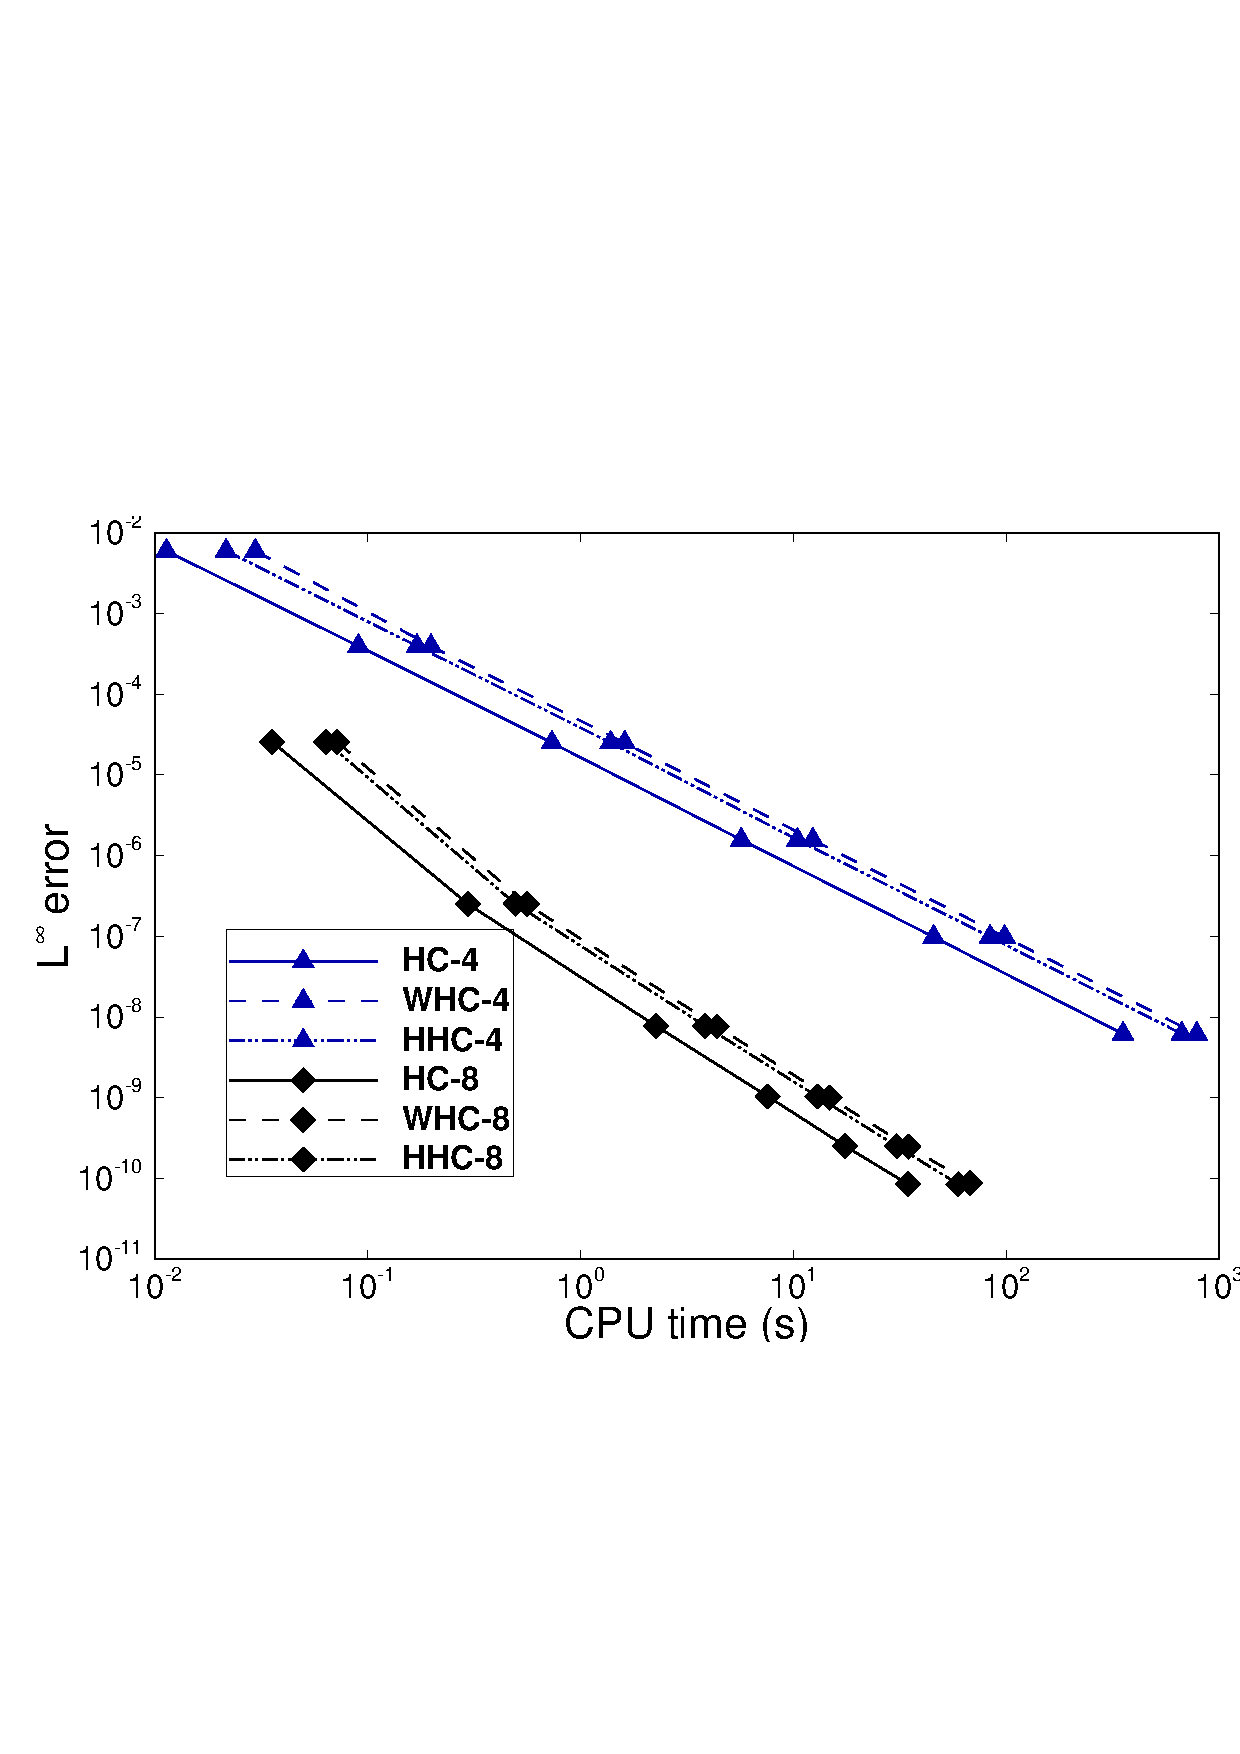
\includegraphics[width=0.8\textwidth]{fig/Time/Time-2D.pdf}
  \caption{几种数值格式在\cref{ex:2D-acc2-re} 中CPU时间与密度的$L^\infty$误差之间的关系。
    本图中所有格式的CFL数均取0.5。
  }
  \label{fig:2D-time}
\end{figure}

\section{小结}

本章针对二维双曲守恒律,
设计了基于紧致埃尔米特重构的两步四阶数值格式。
具体地说,
我们经过对模板的精心挑选,
成功得到真正的二维线性紧致埃尔米特重构,
并设计了相应的线性格式。
这些二维重构在一维问题中可以退化到我们先前构造的一维重构,
从而这些二维重构可以取得类似一维重构的良好性能。
然后,
基于二阶和四阶的线性重构,
我们构造了两种四阶精度基本无振荡的非线性重构,
即加权型和杂交选择型的紧致埃尔米特重构,
并设计了相应的时空四阶精度基本无振荡的两步四阶格式。
它们均采用二维的Godunov解法器和二维弱耦合的广义黎曼问题解法器。
我们也将格式推广到了空间八阶精度。
接着,
我们讨论了数值格式的紧致性,
得出了结论:与文\cite{du2018hermite}中的二维两步四阶格式相比,
我们的二维四阶精度两步四阶格式更加紧致。
最后我们给出了许多算例,
验证了我们的数值格式具有高精度、稳定、紧致、高效以及基本无振荡的优良特性。